\DeclarePairedDelimiter\norm{\lVert}{\rVert}

\section{Creature Generation}
\subsection{Parametrische Kreatur}
Als Grundlage für die parametrische Generierung der Kreaturen dient das von Jon Hudson in seiner Thesis \cite{Hudson2013CreatureGU} beschriebene Modell, welches in Abschnitt \ref{} näher beschrieben wird.\\
Die Kreatur besteht aus mehreren Körperteilen, die separat generiert werden und jeweils ihre eigenen Parameter besitzen. Diese Körperteile sind Torso, Beine, Arme, Hals, Füße und Kopf, die jeweils aus einem oder mehreren Knochen bestehen. Alle in diesem Abschnitt erwähnten Zufallsvariablen entstammen einer uniformen Verteilung.

\subsubsection{Knochen Koordinaten}
Um einfache lokale Transformationen zu ermöglichen, definieren wir ein einheitliches Koordinatensystem für alle Knochen. Der Ursprung dessen ist der \textbf{proximale Punkt}, dieser ist der der Körpermitte am nächsten gelegene Punkt und entspricht somit der Stelle, an der der knochen, gegebenenfalls mit einem Offset, an seinem Elternknochen befestigt ist. Der \textbf{distale Punkt} ist der Endpunkt des Knochens, also der am weitesten von der Körpermitte entfernte Punkt. \\ Die \textbf{proximale Achse} verläuft parallel zum Knochen, von der Körpermitte weg, also in Richtung des distalen Punktes. Die \textbf{ventrale Achse} liegt orthogonal zur proximalen Achse und zeigt in Richtung der Vorderseite des Knochens. Diese lässt sich prinzipiell beliebig definieren, in unserem Fall haben wir uns jedoch für Armknochen auf die dem Körper zugewandte Innenseite des Knochens festgelegt, für parallel zum Boden generierte Torsi auf die Unterseite und für alle weiteren Knochen auf die der Blickrichtung des Skeletts zugewandten Seite. Die \textbf{laterale Achse} liegt senkrecht auf den beiden zuvor definierten Achsen.

\subsubsection{Generierung}
Unsere Methode setzt voraus, dass zunächst gewisse Vorgaben zur generellen Struktur der Kreatur gemacht werden. In unserem konkreten Fall bedeutet dies, dass wir uns zunächst auf Zwei- und Vierbeiner beschränken. Der Zweibeiner orientiert sich an der menschlichen Anatomie und besitzt deshalb in jedem Bein jeweils zwei Knochen und einen einzelnen Fußknochen sowie zwei Arme. Die Beine eines Vierbeiners besitzen, angelehnt an die Skelette echter vierbeiniger Säugetiere, jeweils vier Knochen. Arme werden hier nicht generiert. Um Kreaturen zu erzeugen, die nicht einer dieser Strukturen entsprechen, wie beispielsweise Spinnentiere oder Echsen, müsste man weitere Skelette definieren.\\
\\
Zuerst  wird der \textbf{Torso} Generiert. Im Falle des Zweibeiners ist dieser nach oben gerichten, beim Vierbeiner parallel zum Boden. Als Parameter werden jeweils Minima und Maxima für die Länge und den Umfang des Torsos übergeben. Daraus wird zunächst ein zufälliger Wert für die Länge bestimmt. Da wir uns vorerst für einen Torso bestehend aus drei Knochen entschieden haben, wird diese Länge zufällig auf drei kleinere Längen aufgeteilt. Jeder dieser Knochen erhält dann einen zufälligen Umfang. Das unterste Torsosegment dient als Elternknochen der Kreatur, die anderen beiden Knochen werden dann nacheinander am distalen Punkt des vorangegangenen Knochens befestigt.\\
Anschließend werden die \textbf{Beine} paarweise generiert, wodurch nur symmetrische Kreaturen erstellt werden können. Auch hier wird zunächst die Länge zufällig bestimmt und dann auf zwei beziehungsweise vier Knochen aufgetelt. Auch Die Umfänge werden zufällig bestimmt, jedoch zusätzlich sortiert, sodass das das dickste Segment der Körpermitte am nächsten gelegen ist. In beiden Fällen werden die Beine gerade nach unten gereriert. Bei einem Zweibeiner wird am distalen Punkt des unteren Beinknochen in Richtung dessen ventraler Achse ein Fußknochen mit parametrisch zufällig bestimmter Größe erzeugt. Befestigt werden die Beine durch einen zusätzlichen Hüftknochen, der parallel zum Torso am proximalen Punkt des ersten Torsoknochens ansetzt und dessen proximale Achse entgegen derer seines Elternknochens gerichtet ist, also den Torso etwas verlängert. Es wird jeweils ein Bein links und rechts vom Mittelpunkt des Hüftknochens angebracht. Der Abstand entlang der lateralen Achse ergibt sich aus dem Umfang des Knochens. Im Falle des Vierbeiners wird analog dazu ein weiteres Beinpaar am distalen Punkt des letzten Torsoknochens generiert. Anschließend werden Torso und Beine so rotiert, dass sich alle Enden der Beine auf der selben Höhe befinden und die Beine noch immer gerade nach unten Zeigen.\\
Die \textbf{Arme} des Zweibeiners werden analog zu den Beinen mit Hilfe eines Schultersegmentes am distalen Punkt des obersten Torsoknochens erzeugt.\\
Der \textbf{Hals} wird als Verlängerung des Torsos generiert. Dabei wird sowohl die Länge und Dicke zufällig bestimmt als auch die Anzahl der Knochen. Beim Zweibeiner wird er am distalen Punkt des Schulterknochens befestigt und alle Knochen zeigen parallel zum Torso gerade nach oben. Beim Vierbeiner erfolgt das Befestigen am distalen Punkt des vorderen Hüftknochens. Dabei ist die Rotation des ersten Knochens ein zufälliger Wert zwischen der der proximalen und der der negativen ventralen Achse des Elternknochens. Jedes weitere Halssegment erhält eine zufällige Rotation um $\pm 20\degree$.\\
Der \textbf{Kopf} ist ein einzelner Knochen mit zufälliger Länge und Umfang, der als Verlängerung des letzten Halsknochens betrachtet werden kann.\\
\\
Die glaubwürdigkeit und Variation der Kreaturen ist dadurch also auch stark von den gewählten Parametern Abhängig. Diese werden von Hand gesetzt, wobei größere Wertebereiche auch für größere Unterschiede zwischen den Kreaturen sorgen, aber gleichzeitig die Kontrolle über das Ergebnis einschränken. Die Beschränkungen der Bewegungsradii der Gelenke werden momentan händisch mit erfahrungsgemäß guten Werten gesetzt. Ziel ist es allerdings auch diese in Zukunft soweit möglich prozedural mit Hilfe von Parametern zu erzeugen, um verschiedene Bewegungsmuster zu ermöglichen.




\subsection{L-System Creature}
% Vom L-System zu den Knochen (Strecken) -> Rotation um die Achsen mittels Euler->Quarternion
\subsubsection{Generierung der Skelettstruktur}



\subsection{Metaballs}
Zur Generierung der Geometrie der Kreatur verwenden wir, angelehnt an den Ansatz von Madis Janno \cite{Janno20182dCG} (siehe \ref{}), eine modifizierte Form von Metaballs. Wie auch bei Janno lässt sich unsere Methode mit beliebigen Metaball-Funktionen durchführen. Aufgrund der guten Ergebnisse haben wir uns jedoch vorerst auf die gleiche, zuerst von Ken Perlin beschriebene, Falloff-Funktion festgelegt.
\[f_i(x,y,z) = exp(B_i - \frac{B_ir_i^2}{R_i^2} - B_i)\]
Für Metaball $i$ ist $r_i$ der Abstand des Punktes $(x,y,z)^T$ zu dessen Zentrum, also: \[r_i=||(x,y,z)^T-(x_i,y_i,z_i)^T||_2=\sqrt{(x-x_i)^2+(y-y_i)^2+(z-z_i)^2}\]
$R_i$ ist der Radius von Metaball $i$ und $B_i$ ein Parameter zur Einstellung der "Blobbiness". Wir verwenden Werte mit $B_i < 0.5$. \\
Die generierten Kreaturen bestehen aus mehreren Segmenten (Knochen) mit jeweils einem Start- und Endpunkt sowie einer Dicke, die als Radius der darauf platzierten Metaballs verwendet werden kann. Entlang dieser Segmente soll dann das Mesh erzeugt werden. Die von Janno beschriebene Methode berechnet dafür, abhängig von der gewählten Falloff-Funktion, die minimale Anzahl an Metabällen für ein Segment und platziert diese gleichmäßig entlang dessen. Das Problem, welches sich daraus bei unseren Experimenten ergeben hat, liegt darin, dass mit höherer Komplexität der Kreaturen und einer damit einhergehenden steigenden Anzahl an Segmenten, der Einfluss von benachbarten Segmenten nicht gut kontrollieren lässt und diese teilweise ineinander verschmelzen. \\

Unser Ansatz um dieses Problem zu umgehen ist es, die Anzahl der einzelnen Metabälle drastisch zu reduzieren. Anstatt einer beliebig großen Zahl an Bällen entlang jedes Segments, erzeugen wir jeweils nur einen einzigen. Dazu ersetzen wir die Bälle durch Kapseln, also Zylinder mit jeweils durch eine Halbkugel abgerundeten Enden. Möglich macht uns dies eine Modifikation der Falloff-Funktion, beziehungsweise der darin verwendeten Distanz. Wir berechnen hierbei nicht den Abstand zum Zentrum einer Kugel, sondern zu der Verbindungslinie zwischen Start- und Endpunkt. \\

\begin{figure}[ht]
\centering
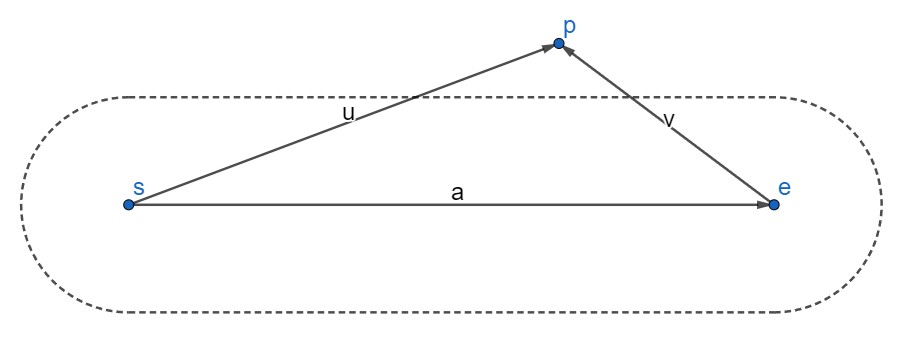
\includegraphics[width=0.7\textwidth]{resources/img/metacapsule.png}
\caption{Beispiel Metakapsel; Die gestrichelte Linie enthält alle Punkte mit $r=R$}
\label{metacapsule}
\end{figure}

Sei $s$ der Startpunkt, $e$ der Endpunkt, $a$ der Vektor $e-s$, $p$ ein Punkt, dessen Abstand berechnet werden soll, $u=p-s$ und $v=p-e$ (Siehe Abbildung \ref{metacapsule}). Die Distanz lässt sich dann folgendermaßen bestimmen:
\[
    r= 
\begin{cases}
    ||p-s||,& \text{falls } a\cdot u < 0\\
    ||p-e||,& \text{falls } a\cdot v > 0\\
    \norm*{\frac{a\times u}{\norm{a}}},& \text{sonst}
\end{cases}
\]

Es werden drei Fälle unterschieden. Liegt der Punkt $p$ im Falle von Abbildung \ref{metacapsule} links von $s$, beziehungsweise rechts von $e$, ist Die Distanz von $p$ zum Segment einfach der euklidische Abstand zum jeweiligen Punkt. Ob dies der Fall ist, lässt sich mit Hilfe der Skalarprodukte $a\cdot u$ beziehungsweise $a\cdot v$ überprüfen. Ansonsten berechnet man die Distanz von Punkt p zur Geraden, die durch $s$ und $e$ verläuft.\\

Da dies nur eine Erweiterung der Metaball-Funktion ist, lassen sich diese Kapseln weiterhin mit anderen Metabällen kombinieren. So können auch Körperteile erstellt werden, die nicht aus solchen Segmenten bestehen, oder Details aus kleineren Metabällen entland der Segmente platziert werden.



\subsection{Marching Cubes / Mesh Generation}



\subsection{Automatic Rigging}
